%% abtex2-modelo-trabalho-academico.tex, v-1.9.2 laurocesar
%% Copyright 2012-2014 by abnTeX2 group at http://abntex2.googlecode.com/ 
%%
%% This work may be distributed and/or modified under the
%% conditions of the LaTeX Project Public License, either version 1.3
%% of this license or (at your option) any later version.
%% The latest version of this license is in
%%   http://www.latex-project.org/lppl.txt
%% and version 1.3 or later is part of all distributions of LaTeX
%% version 2005/12/01 or later.
%%
%% This work has the LPPL maintenance status `maintained'.
%% 
%% The Current Maintainer of this work is the abnTeX2 team, led
%% by Lauro César Araujo. Further information are available on 
%% http://abntex2.googlecode.com/
%%
%% This work consists of the files abntex2-modelo-trabalho-academico.tex,
%% abntex2-modelo-include-comandos and abntex2-modelo-references.bib
%%

% ------------------------------------------------------------------------
% ------------------------------------------------------------------------
% abnTeX2: Modelo de Trabalho Academico (tese de doutorado, dissertacao de
% mestrado e trabalhos monograficos em geral) em conformidade com 
% ABNT NBR 14724:2011: Informacao e documentacao - Trabalhos academicos -
% Apresentacao
% ------------------------------------------------------------------------
% ------------------------------------------------------------------------

\documentclass[
    % -- opções da classe memoir --
    12pt,               % tamanho da fonte
    openright,          % capítulos começam em pág ímpar (insere página vazia caso preciso)
    twoside,            % para impressão em verso e anverso. Oposto a oneside
    a4paper,            % tamanho do papel. 
    % -- opções da classe abntex2 --
    %chapter=TITLE,     % títulos de capítulos convertidos em letras maiúsculas
    %section=TITLE,     % títulos de seções convertidos em letras maiúsculas
    %subsection=TITLE,  % títulos de subseções convertidos em letras maiúsculas
    %subsubsection=TITLE,% títulos de subsubseções convertidos em letras maiúsculas
    % -- opções do pacote babel --
    english,            % idioma adicional para hifenização
    french,             % idioma adicional para hifenização
    spanish,            % idioma adicional para hifenização
    brazil              % o último idioma é o principal do documento
    ]{abntex2}

% ---
% Pacotes básicos 
% ---
\usepackage{lmodern}            % Usa a fonte Latin Modern          
\usepackage[T1]{fontenc}        % Selecao de codigos de fonte.
\usepackage[utf8]{inputenc}     % Codificacao do documento (conversão automática dos acentos)
\usepackage{lastpage}           % Usado pela Ficha catalográfica
\usepackage{indentfirst}        % Indenta o primeiro parágrafo de cada seção.
\usepackage{color}              % Controle das cores
\usepackage{graphicx}           % Inclusão de gráficos
\usepackage{microtype}          % para melhorias de justificação
% ---

\usepackage{xcolor}
\usepackage{listings}  
\lstset { %
	numbers=left,
    language=java,
    escapeinside={\%*}{*)},
    backgroundcolor=\color{black!5},
	basicstyle=\ttfamily\scriptsize,
    keywordstyle=\color{blue}\ttfamily,
    stringstyle=\color{red}\ttfamily,
    commentstyle=\color{red}\ttfamily,
    breaklines=true,
    morecomment=[l][\color{magenta}]{\#}
}
\lstdefinelanguage{XML}
{
  %morestring=[b]",
  morestring=[s]{>}{<},
  morecomment=[s]{<?}{?>},
  stringstyle=\color{black},
  identifierstyle=\color{blue},
  keywordstyle=\color{cyan},
	showstringspaces=false,
  morekeywords={xmlns,version,type}% list your attributes here
}
\usepackage{pdflscape}
\usepackage{float}
\usepackage{subfigure}

\renewcommand{\lstlistingname}{Listagem}
    
% ---
% Pacotes adicionais, usados apenas no âmbito do Modelo Canônico do abnteX2
% ---
\usepackage{lipsum}             % para geração de dummy text
% ---

% ---
% Pacotes de citações
% ---
\usepackage[brazilian,hyperpageref]{backref}     % Paginas com as citações na bibl
\usepackage[alf]{abntex2cite}   % Citações padrão ABNT

% --- 
% CONFIGURAÇÕES DE PACOTES
% --- 

% ---
% Configurações do pacote backref
% Usado sem a opção hyperpageref de backref
%\renewcommand{\backrefpagesname}{Citado na(s) página(s):~}
% Texto padrão antes do número das páginas
%\renewcommand{\backref}{}
% Define os textos da citação
%\renewcommand*{\backrefalt}[4]{
%    \ifcase #1 %
%        Nenhuma citação no texto.%
%    \or
%        Citado na página #2.%
%    \else
%        Citado #1 vezes nas páginas #2.%
%    \fi}%
% ---

% ---
% Informações de dados para CAPA e FOLHA DE ROSTO
% ---
\titulo{Modelo Canônico de\\ Trabalho Acadêmico com \abnTeX}
\autor{Equipe \abnTeX}
\local{Brasil}
\data{2014, v-1.9.2}
\orientador{Lauro César Araujo}
\coorientador{Equipe \abnTeX}
\instituicao{%
  Universidade do Brasil -- UBr
  \par
  Faculdade de Arquitetura da Informação
  \par
  Programa de Pós-Graduação}
\tipotrabalho{Tese (Doutorado)}
% O preambulo deve conter o tipo do trabalho, o objetivo, 
% o nome da instituição e a área de concentração 
\preambulo{Modelo canônico de trabalho monográfico acadêmico em conformidade com
as normas ABNT apresentado à comunidade de usuários \LaTeX.}
% ---


% ---
% Configurações de aparência do PDF final

% alterando o aspecto da cor azul
\definecolor{blue}{RGB}{41,5,195}

% informações do PDF
\makeatletter
\hypersetup{
        %pagebackref=true,
        pdftitle={\@title}, 
        pdfauthor={\@author},
        pdfsubject={\imprimirpreambulo},
        pdfcreator={LaTeX with abnTeX2},
        pdfkeywords={abnt}{latex}{abntex}{abntex2}{trabalho acadêmico}, 
        colorlinks=true,            % false: boxed links; true: colored links
        linkcolor=blue,             % color of internal links
        citecolor=blue,             % color of links to bibliography
        filecolor=magenta,              % color of file links
        urlcolor=blue,
        bookmarksdepth=4
}
\makeatother
% --- 

% --- 
% Espaçamentos entre linhas e parágrafos 
% --- 

% O tamanho do parágrafo é dado por:
\setlength{\parindent}{1.3cm}

% Controle do espaçamento entre um parágrafo e outro:
\setlength{\parskip}{0.2cm}  % tente também \onelineskip

% ---
% compila o indice
% ---
\makeindex
% ---
\graphicspath{{images/}} %Pasta padrão das imagens
% ----
% Início do documento
% ----
\begin{document}

  %\pagestyle{empty}
	%Arquivo de Capa
\newpage
\begin{figure}[!htp]
  
\includegraphics[scale = 0.4]{unesp-logo.png}  %logo da UNESP
\end{figure}

\hspace*{73mm}
\begin{minipage}{79mm}
	\vskip-35mm
	\begin{center}
		UNIVERSIDADE ESTADUAL PAULISTA \\[-2mm] "JÚLIO DE MESQUITA FILHO" \\[-2mm] Campus de Presidente Prudente
	\end{center}
\end{minipage}
\begin{center}
	{\large Fundação de Amparo à Pesquisa do Estado de São Paulo (FAPESP)  }
\end{center} 
%nome do autor
\vspace*{30mm}
\begin{center}
	{\large Uso de \textit{Business Process Model} como apoio à condução e à replicação de experimentos controlados em Engenharia de Software 
  }
\end{center}

\vspace*{15mm}

\begin{center}
	{\large RELATÓRIO CIENTÍFICO FINAL \\ (Pedido de renovação da bolsa)  }\\
\end{center}



{\flushleft
	{\normalsize
		\vspace{30mm}
		\hrulefill\\
		%\hspace{10mm} \textbf{Título: }Uso de \textit{Business Process Model} como apoio à condução e à replicação de experimentos controlados em Engenharia de Software \\
		\hspace{10mm} \textbf{Bolsista: }Leandro Ungari Cayres\\
		\hspace{10mm} \textbf{Orientador: }Prof. Dr. Rogério Eduardo Garcia\\
		%\hspace{10mm} \textbf{Orgão Financiador: }Fundação de Amparo à Pesquisa do Estado de São Paulo (FAPESP)\\
		\hspace{10mm} \textbf{Processo: }2016/17477-2\\
		\hspace{10mm} \textbf{Período do relatório: }01/06/2017 a 30/09/2017\\
		\hspace{10mm} \textbf{Vigência: }01/12/2016 a 30/11/2017 \\
		\hrulefill\\
	}
}

\vspace*{\fill}

\begin{center}
	Presidente Prudente \\Setembro de 2017  %local da tortura e data da entrega do plágio
\end{center}
	
	%\pagestyle{misc}
  \pagenumbering{roman}
	\textual	
	\tableofcontents 
	\newpage
	\listoffigures 
	\newpage
	\listoftables 
	
	\clearpage
	\pagenumbering{arabic}
	%\textual	
	\chapter{Introdução}

Este relatório tem como objetivo apresentar as atividades desenvolvidas pelo bolsista Leandro Ungari Cayres referente ao projeto  registrado junto à FAPESP com número 2016/17477-2, sob orientação do Prof. Dr. Rogério E. Garcia, período compreendido entre dezembro de 2016 a maio de 2017.

O objetivo geral deste projeto consiste em prover uma interface capaz de apresentar visualmente o protocolo de um experimento, utilizando a notação BPM (\textit{Business Process Modeling}). Ou seja, deve-se: (1) prover ao experimentador a possibilidade de planejar seu experimento utilizando a notação BPM e; (2) prover ao replicador a possibilidade de visualizar o protocolo contido no PL, também utilizando a notação BPM.

Como objetivo específico, considera-se a modificação da camada de apresentação (interface) da ferramenta \textit{OntoExpTool}, incorporando o modelo gráfico BPM à ferramenta, assim como as adequações necessárias na camada de controle. É importante ressaltar que objetiva-se constituir um sistema de software que permita a concepção e a troca de pacotes de laboratórios, para apoiar a condução de experimentos controlados.

Como questões de investigação (em nível de Iniciação Científica), tem-se: o uso de BPM contribui para a definição do protocolo de experimentos? Quais recursos devem ser utilizados para o uso da tecnologia? Como suplantar limitações para a tecnologia a ser utilizada?

Para apresentar as atividades desenvolvidas até o momento, este relatório encontra-se dividido em $5$ capítulos, além desta introdução:

\begin{itemize}

\item No capítulo \ref{cp:engenharia} é apresentada uma breve revisão sobre Engenharia de Software Experimental, com foco em experimentos controlados, para contextualização do projeto de pesquisa.

\item No capítulo \ref{cp:bpmn} é descrito um breve histórico da notação BPM, assim como, apresentando os elementos que compõem este notação.

\item No capítulo \ref{cp:prototipo} é apresentado o andamento das atividades de implementação da interface de modelagem.

\item No capítulo \ref{ch:plano_atividades} é apresentado o plano de atividades inicial para o projeto. É, também, apresentado o que fora cumprido até o presente momento, bem como as atividades que serão efetuadas a partir desta etapa.

\item Por fim, no Capítulo \ref{cp:conclusoes} são apresentadas as considerações finais do presente relatório.
\end{itemize}
     


	
	\chapter{Processo Experimental: seus dados e metadados}
\label{cp:engenharia}

A Engenharia de Software Experimental busca medir e avaliar modelos e tecnologias em contextos práticos, objetivando a obtenção de um corpo de conhecimento. Porém, resultados oriundos de um único experimento não podem estabelecer tal corpo de conhecimento, de modo a determinar fatos sobre um dado fenômeno devido às mais diversas variações que podem ser introduzidas no processo experimental, tais como influências culturais~\cite{Basili99, Miller:2005, Shull03}. Perante a isto, se faz necessário que dados sobre estudos independentes sejam armazenados e compartilhados.

O ato de experimentação consiste no centro do processo científico, a qual representa uma atividade na área de pesquisa científica e se utiliza de métodos de investigação experimental para a condução de experimentos~\cite{Travassos02}. 

Segundo \citeauthoronline{Basili99}~(\citeyear{Basili99}), a experimentação ajuda a determinar a eficácia de métodos e de teorias propostas. Somente experimentos verificam as teorias, podem explorar os fatores críticos, e dar luz ao fenômeno novo para que as teorias possam ser formuladas e corrigidas.

A execução de um experimento requer uma sequência de atividades estabelecidas previamente, que por meio das quais seja possível conduzir um processo experimental de forma precisa e sistemática. Desse modo, \citeauthoronline{Wohlin2012}~(\citeyear{Wohlin2012}) propõem as seguinte organização em fases: 
\begin{itemize}
\item \textbf{Definição} –- estabelece quais são os problemas tratados;
\item \textbf{Planejamento} -– determina-se o projeto, instrumentação e os possíveis riscos para validação dos resultados;
\item \textbf{Operação} –- coleta-se os dados do experimento;
\item \textbf{Análise e Interpretação} –- os dados são analisados e avaliados;
\item \textbf{Apresentação e Empacotamento} -– os resultados são apresentados e suas informações são armazenadas para uso futuro.
\end{itemize}

%\textbf{Definição} -- estabelece quais são os problemas tratados; \textbf{Planejamento} -- determina-se o projeto, instrumentação e os possíveis riscos para validação dos resultados; \textbf{Operação} -- coleta-se os dados do experimento; \textbf{Análise e Interpretação} -- os dados são analisados e avaliados; \textbf{Apresentação e Empacotamento} -- os resultados são apresentados e suas informações são armazenadas para uso futuro. 

Na Figura~\ref{ideia} é apresentado um gráfico com o processo de experimentação adaptado de~\citeauthoronline{Wohlin2012}~(\citeyear{Wohlin2012}): nela é possível observar as fazes, assim como tarefas inerentes a cada uma. 

\begin{figure}[!ht]
\centering
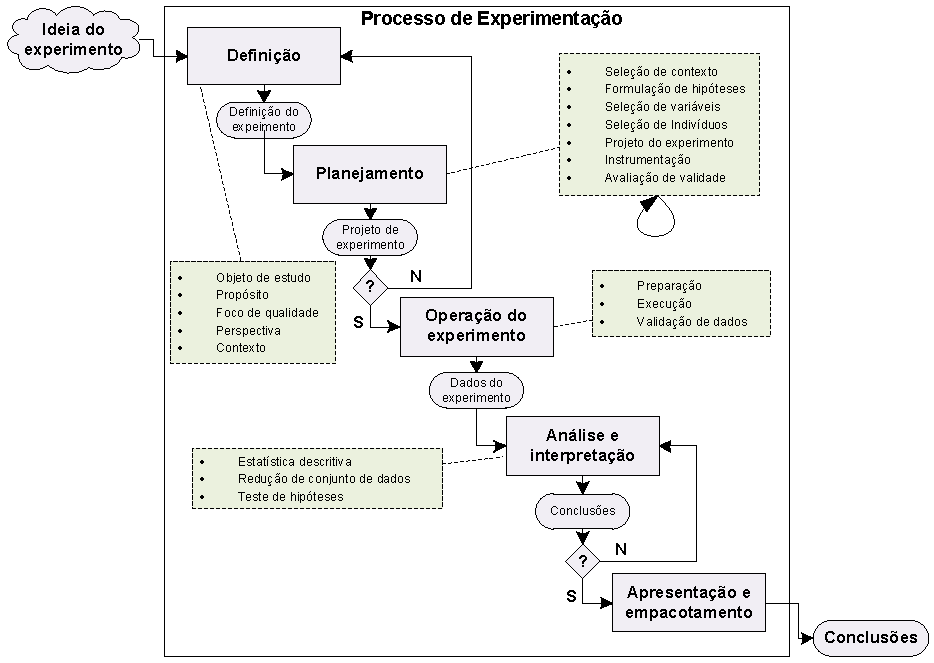
\includegraphics[width=0.98\textwidth]{images/Experimentacao.pdf}
\caption{Processo de Experimentação -- adaptado de~\cite{Wohlin2012}.}
\label{ideia}
\end{figure}

Como apoio, os estudos experimentais atuam como ferramentas para obtenção dos dados necessários através de todo o processo de desenvolvimento de software, almejando resultados objetivos e significativos de forma a alcançar melhorias no processo. Também segundo~\citeauthoronline{Wohlin2012}~(\citeyear{Wohlin2012}), tais estudos podem ser divididos nas seguintes categorias:

\begin{itemize}

\item Pesquisa de opinião: neste primeiro tipo de estudo experimental, busca-se obter dados a respeito de uma técnica ou ferramenta específica, seja uma análise qualitativa ou quantitativa, por meio de entrevistas ou questionários aplicados a uma amostra capaz de representar uma determinada população. Nesta categoria, não controle de execução ou medidas.

\item Estudos de caso: esta categoria é voltada ao monitoramento de atividades, projetos ou tarefas visando observar um atributo específico, ou estabelecer relações entre alguns destes, a qual se prolonga por um determinado período de tempo. Por se tratar uma atividade observacional, o nível de controle é mais elevado do que o anterior.

\item Experimentos controlados: por fim, nesta categoria, o estudo experimental tem sua execução manipulada de forma direta e sistemática, a fim de se ter controle sob todos os elementos que o compõem. Podem ser efetuados experimentos controlados em ambiente universitário, de forma a reduzir custos e riscos do que aplicá-los diretamente à indústria.

\end{itemize}

Somente experimentos verificam as teorias, podem explorar os fatores críticos, e dar luz ao fenômeno novo para que as teorias possam ser formuladas e corrigidas. O processo experimental proporciona de modo sistemático, disciplinado, e controlada a avaliação de processos e de atividades humanas~\cite{Travassos02}.

Através da replicação de experimentos, pesquisadores adquirem conhecimento adicional a respeito dos conceitos estudados. Para que se possa replicar experimentos, é necessário que seu empacotamento seja realizado apropriadamente. Uma replicação em contextos diferentes sujeita o experimento a variações, dentre os quais fatores humanos, socioeconômicos e ambientais do âmbito que o experimento é realizado, possibilitando maior precisão na verificação da validade de hipóteses~\cite{Shull03}. E para a replicação de um experimento, tanto intra quanto extra-grupo~\cite{Mendonca08}, é de suma importância a organização do registro das atividades de um experimento controlado, que são mantidas no chamado \textit{Pacote de Laboratório}.

%%%%%%%%%%%%%%%%%%%%%%%%%%%%%%%%%%%%%%%%
%%%%%%%%%%%%%%%%%%%%%%%%%%%%%%%%%%%%%%%%

\section{Pacotes de Laboratório}
\label{sec:Pacote}
Dentro do âmbito da Engenharia de Software Experimental, a todo momento diversas pesquisas, técnicas e ferramentas são desenvolvidos para validar teses ou otimizar soluções, porém tais recursos ou informações isoladas não formam um corpo de
conhecimento consistente, faz-se necessário compartilhá-los entre os grupos de pesquisa por meio do uso de pacotes de laboratório.

A condução de experimentos controlados ou de suas respectivas replicações, ambas necessitam de validação. A execução destes experimentos, tanto no papel de experimentador quanto de replicador, podem influenciar de forma positiva ou negativa sob muitos aspectos, principalmente em relação ao nível de experiência do condutor do experimento. Por fim, o conjunto de informações obtidos através da execução do processo experimental compõem uma nova instância de pacote de laboratório~\cite{Garcia08}.

Diversos pesquisadores relatam dificuldades na revisão de pacotes de laboratório, como problemas no compartilhamento de conhecimento entre grupos de pesquisa devido uma falta de padronização para a integração de um conhecimento novo e/ou isolado ao conhecimento comum~\cite{Scatalon11}. Desta forma, é imprescindível uma boa definição e construção
de um pacote de laboratório com o uso de uma estrutura específica de simples compreensão, possibilitando inclusive o uso de ontologias para seu desenvolvimento.


%Garcia et al. 
\citeauthoronline{Garcia08} (\citeyear{Garcia08}) propõem o uso de uma ontologia para apoiar a atividade de \textit{Empacotamento} processo de Experimentação no contexto de Engenharia de Software, que descreve os conceitos que compõem um pacote de laboratório para experimentos controlados, chamada \textit{ExperOntology}, apresentada na Figura~\ref{fig:onto01}.
Uma ontologia é uma especificação formal explícita de uma conceitualização compartilhada, definindo parte de um domínio por meio de termos relevantes e seus respectivos relacionamentos, cuja estruturação é baseada por determinadas regras. As regras (axiomas) da \textit{ExperOntology} não são apresentados aqui, mas podem ser observados em~\cite{Garcia08}.
\begin{figure}[!ht]
\centering
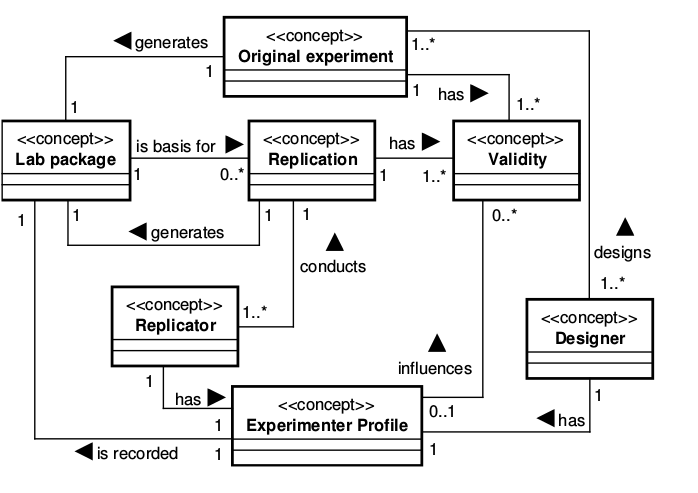
\includegraphics[width=0.8\textwidth]{images/controlados.png}
\caption{Ontologia para Experimentos Controlados~\cite{Garcia08}.}\label{fig:onto01}
\end{figure}

\begin{figure}[!htb]
\centering
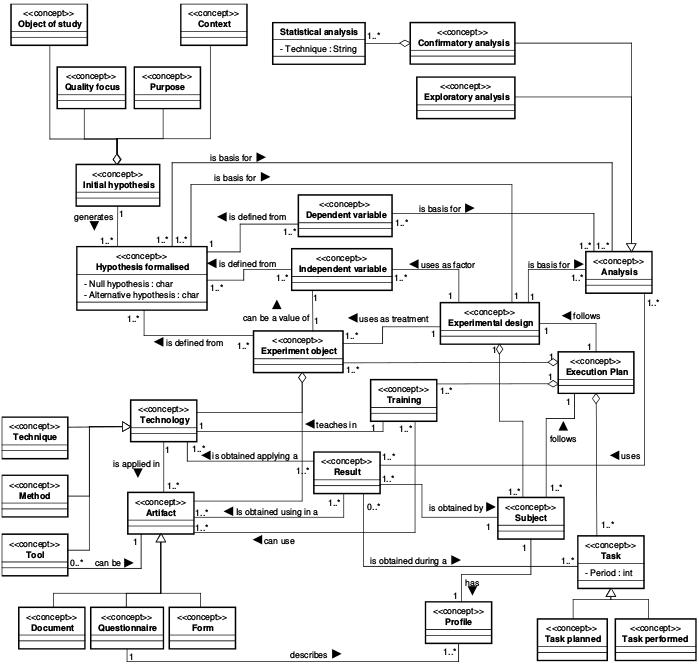
\includegraphics[width=\textwidth]{images/onto.png}
\caption{Ontologia para Pacotes de Laboratório~\cite{Garcia08}.}\label{fig:onto02}
\end{figure}

A \textit{ExperOntology} visa a definir o principais conceitos de experimentos controlados desde a fase de definição até a análise de resultados, sendo importante ressaltar a evolução do experimento e o uso de pacotes de laboratório para armazenamento~\cite{Garcia08}. 

Na Figura \ref{fig:onto02} estão descritos os conceitos que devem fazer parte de um pacote de laboratório, segundo a \textit{ExperOntology}. Inicialmente, é definido um propósito, um contexto, um objeto de estudo e o foco a serem considerados no estudo controlado; en seguida, é elaborada de uma hipótese inicial, a qual juntamente com uma objeto de estudo e um contexto formam a formalização da hipótese. A partir deste ponto, são definidas as hipóteses nulas e alternativas, assim como as variáveis dependentes e independentes. Durante a fase de planejamento, são determinados os objetos de experimentação como as tecnologias e artefatos sob investigação.

O principal objetivo das fases de definição e planejamento é estabelecer um modelo experimental que satisfaça todos os requisitos para a fase de análise. O resultado destas fases culmina em um modelo experimental e no plano de execução, o qual permite a definição de um ambiente controlado, realização de testes das hipóteses e minimização de ameaças para a validação do experimento.

Todos os conceitos apresentados devem ser mantidos no Pacote de Laboratório e, portanto, devem ser instanciados em uma base de dados ou outro meio equivalente para persistir os dados.

\section{Bancos de Dados Não-Relacionais}

Diversas tecnologias para armazenamento de dados têm sido propostas para a persistência de dados, como os Sistemas Gerenciadores de Banco de Dados (\textit{SGBDs}).

O modelo relacional de dados tem sido utilizado em larga escala desde a sua criação. Este modelo tem como característica a utilização de tabelas e tuplas para o armazenamento de dados, assim como o uso de chaves primárias para garantia de unicidade (identificação única de elementos de dados)~\cite{brito2010bancos}.

Mediante ao crescente número de aplicações, o volume de dados tem aumentado exponencialmente nos últimos anos, e com tal crescimento limitações do modelo relacional tem ficado evidente, principalmente quanto à eficiência na recuperação de dados e escalabilidade~\cite{toth2011abordagem}. Para este projeto, a principal limitação é a necessidade de se ter uma estrutura de tabelas pré-definidas, com seus respectivos atributos, o que pode ser uma restrição, pois experimentos controlados podem ter variações nos dados tratados, difícil de ser acomodados em uma estrutura relacional.

Como alternativa, há soluções tecnológicas alternativas que priorizam flexibilidade quanto ao armazenamento, desse modo, não empregam regras presentes no modelo relacional tradicional. Um dessas alternativas é o Modelo Não-Relacional (NoRel), o qual não tem como objetivo substituir o modelo relacional por completo, mas somente em casos em que seja mais vantajoso utilizá-lo, como em ambientes de Big Data. Alguns representantes de base não-relacionais são: Cassandra~\cite{cassandra2014apache}, Dynamo~\cite{sivasubramanian2012amazon}, MongoDB~\cite{banker2011mongodb} e BigTable~\cite{chang2008bigtable}.

Devido à inexistência de regras para a organização dos seus dados, diversas categorias de sistemas de banco de dados não-relacionais tem sido desenvolvidas, os principais são detalhados a seguir.


\begin{itemize}
\item Orientados a Colunas (\textit{Column}): é a categoria que mais se aproxima do modelo relacional, porém todas as suas operações são voltadas para as colunas, ao invés das tuplas como no modelo relacional. O seu grande diferencial está na facilidade de inserção de novas colunas, ou seja, atributos com o sistema já em operação, conforme se tornarem necessários, sem apresentar problemas de esquema ou redundância de dados~\cite{vaish2013getting}.

\item Armazenamento em Documentos (\textit{Document}): nesta categoria cada item é armazenado em um novo arquivo, em geral sua organização é feita através de estruturas chamadas coleções as quais são equivalentes as tabelas no modelo relacional, não possuem qualquer esquema, dois objetos de uma mesma coleção podem ter atributos diferentes, o que permite grande flexibilidade, sendo que cada registro é um arquivo. Os principais formatos de arquivos são JSON, XML, BSON e YAML~\cite{vaish2013getting}.

\item Armazenamento Chave/Valor (\textit{Key/Value}): também muito semelhante à categoria anterior (\textit{Document}), porém seu armazenamento é feito com uso de uma chave, assemelhando-se a uma tabela \textit{Hash}, ou um \textit{array} associativo. Sua grande vantagem é busca por chaves~\cite{vaish2013getting}.

\item Armazenamento em Grafos (\textit{Graph}): esta categoria tem foco nos relacionamentos entre as entidades, que no caso são os nós do grafo, permitindo o uso de múltiplas ligações entre os nós para demonstrar características em comum. Este modelo pode ser ideal para redes sociais. Uma prática usual é a mescla entre o banco de dados orientado a documentos e o orientado a grafos, tornando não obrigatória a presença de relacionamentos~\cite{vaish2013getting}.

\end{itemize}

\begin{table}[!htb]
\centering
\caption{Banco de Dados Não-Relacional e sua tecnologia de armazenamento.}\label{tab:01}
\begin{tabular}{c|c|c|c|c}
\hline
\textbf{Document} & \textbf{Key-Value} & \textbf{XML} & \textbf{Column} & \textbf{Graph}\\ 
\hline                               
MongoDB & Redis & BaseX & BigTable & Neo4J \\
\hline
CouchDB & Membase & eXist & Haddop/HBase & FlockDB \\
\hline
RavenDB & Voldemort & - & Cassandra & InfiniteGraph \\
\hline
\end{tabular}
\end{table}
\normalsize

Na Tebela~\ref{tab:01} há uma breve lista de tecnologias de banco de dados não-relacionais e a respectiva classificação, segundo as classes de armazenamento apresentadas.
Antes de se estabelecer uma comparação entre os modelos, é importante definir conceitos como que deem compor essa comparação, são eles:



\begin{itemize}
\item Escalonamento: este conceito, no contexto de banco de dados, consiste na capacidade em que uma base de dados tem de destruição tanto horizontal (\textit{scale out}), neste caso a estruturação do sistema é dividida em várias máquinas tanto por parte do banco de dados; quanto vertical (\textit{scale up}), no qual são realizadas melhorias de hardware em relação à processamento e armazenamento~\cite{toth2011abordagem}.

\item Consistência: refere-se à capacidade de manter os dados de forma íntegra, de modo que evite quaisquer problemas no banco de dados possam modificar ou corromper os dados armazenados~\cite{brito2010bancos}.

\item Disponibilidade: este quesito se refere a capacidade de acesso do usuário a referida informação, tanto em quesito de velocidade quanto de solicitação~\cite{brito2010bancos}.
\end{itemize}

\begin{table}[!bth]
\label{comparativo}
\centering
\caption{Análise Comparativa do Modelo Relacional e Não-Relacional~\cite{brito2010bancos}.}
\begin{tabular}{l|p{5.7cm}|p{5.7cm}}
\hline
 & \textbf{Relacional} & \textbf{Não-Relacional} \\ 
\hline                               
\textbf{Escalonamento} & Possível, porém complexo devido à natureza estruturada do modelo, a adição de forma dinâmica e transparente de novos nós no modelo não é realizada de modo natural. & Uma das principais vantagens desse modelo, por não possuir nenhum tipo de esquema predefinido, o modelo possui maior flexibilidade o que favorece a inclusão transparente de outros elementos.\\
\hline
\textbf{Consistência} & Ponto mais forte do modelo relacional. As regras de consistência presentes propiciam uma maior grau de rigor quanto à consistência das informações. & Realizada de modo eventual no modelo: só garante que, se nenhuma atualização for realizada sobre o item de dados, todos os acessos a esse item devolvem o último valor atualizado. \\
\hline
\textbf{Disponibilidade} & Dada a dificuldade de se conseguir trabalhar de forma eficiente com a distribuição dos dados, esse modelo pode não suportar a demanda muito grande de informações do banco. & Outro fator fundamental do sucesso desse modelo. O alto grau de distribuição dos dados propicia que um maior número de solicitações aos dados seja atendida por parte do sistema e que o sistema fique menos tempo não-disponível. \\
\hline
\end{tabular}
\normalsize
\end{table}

Por fim, de modo a esclarecer as reais vantagens e desvantagens do uso de uma base de dados não-relacional, na Tabela~\ref{comparativo} é apresentado um comparativo com o tradicional modelo relacional analisando os quesitos de consistência, escalonamento e disponibilidade~\cite{brito2010bancos}.

Perante esta conceituação, a camada de persistência será elaborada utilizando o banco de dados \textit{MySQL}~\cite{mysql2001mysql} devido à utilização da ferramenta \textit{OntoExpTool}~\cite{Pucci2014}, mantendo assim a compatibilidade para os modelos já criados. Para a persistência da camada de interface será utilizada uma estrutura orientada a documentos, utilizando \textit{eXtensible Markup Language} (XML). Tal decisão foi tomada pois a estrutura orientada a documentos  se mostrou adequada tanto para o armazenamento, quanto para a transferência de protocolos experimentais entre exterimentador e replicador. Adicionalmente, essa organização estrutural permite que os dados de um experimentos sejam mantidos em uma base de dados. e seu protocolo, expresso em BPMN (armazenado em XML) possa ser compartilhado, sem expor os dados. O compartilhamento do protocolo juntamente com os dados do experimento (dados coletados) podem ser compartilhados, desde que desejado pelo experimentador (resposável pela criação do experimento e, consequentemente, do seu Pacote de Laboratório).

	
	\chapter{Modelagem de Processo de Negócio}
\label{cp:bpmn}

Para a elaboração dos modelos de processos de negócio, é relevante o conhecimento de todos os elementos envolvidos na execução de processos, tais como atores, clientes internos e externos, recursos e limitações; por meio dos quais é estabelecido um modelo que propicia um melhor entendimento, organização e representação, seja esta uma visão contextual abstrata ou com alto nível de detalhamento, conforme necessário. 

Tipicamente, a representação de um modelo de processos inclui ícones, que representam atividades, eventos, decisões, condições e outros elementos do processo \cite{brazil2011bpm}. Esses elementos podem conter informações sobre os relacionamentos entre eles e com o ambiente, bem como sobre o comportamento de cada elemento na cadeia de processos.

\section{\textit{Business Process Modeling and Notation}}

A especificação da notação BPMN foi elaborada e lançada em 2004 pelo Instituto de Gerenciamento de Processos de Negócio ou BPMI (\textit{Business Process Management Institute}), que realizou fusão ao Consórcio OMG. Posteriormente, a notação BPMN foi adotada pelo Consórcio OMG como o padrão para modelagem de processos. Após a padronização, foram lançadas algumas versões subsequentes, atualmente encontrando-se na versão 2.0 \cite{object2016business}.

Segundo \citeauthoronline{correia2015enhancing}~(\citeyear{correia2015enhancing}), \textit{Business Process Modeling and Notation} (BPMN) é atualmente a notação de modelagem de processos de negócio mais usada entre profissionais da área, devido a sua flexibilidade e abrangência. Consiste em uma tecnologia recente e pode ser utilizada por profissionais com diferentes níveis de conhecimento técnico. A formalização dos conceitos de modelagem de processos de negócio é baseada em um metamodelo construído a partir da linguagem \textit{Unified Modeling Language} (UML). 

A construção de processos de negócio através desta notação, utiliza um conjunto de padrões denominado ``metamodelo para definição de processos de negócio'' \cite{object2016business}. Nesse sentido, a especificação BPMN provê uma notação gráfica para representar processos de negócio por meio de um diagrama chamado ``diagrama de processo de negócio''. Esse diagrama é elaborado a partir de um conjunto de elementos gráficos que compõem diagramas simples de serem desenvolvidos e
compreendidos. 

\begin{figure}[!ht]
\centering
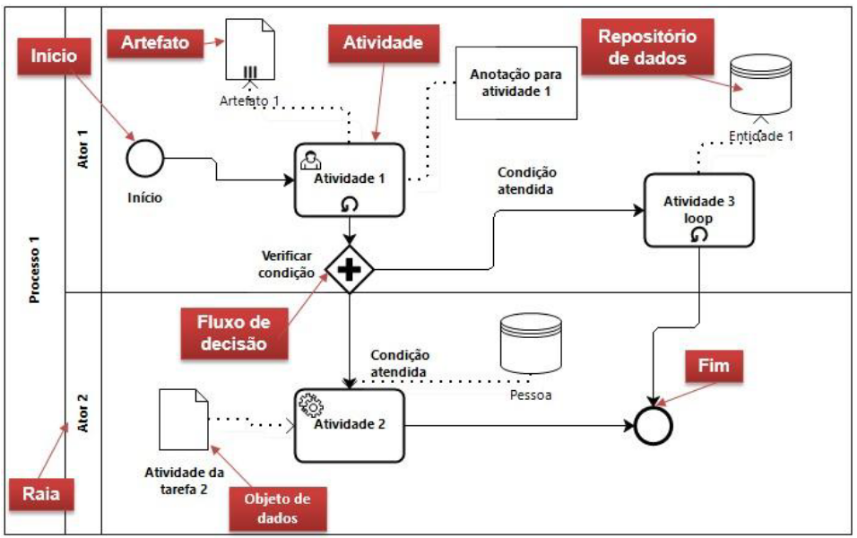
\includegraphics[scale=0.5]{images/diagrama.png}
\caption{Exemplo de diagrama BPMN – adaptado de \cite{Weske2012}.}
\label{diag}
\end{figure}

A Figura \ref{diag} apresenta, como exemplo, um simples diagrama de processo de negócio, através do qual é possível identificar a interação entre dois atores através da execução de atividades e trocas de mensagens, assim como, o uso de recursos como artefatos e repositórios de dados.

A especificação completa da atual versão define atributos que são agrupados em quatro categorias básicas de elementos: objetos de fluxo (\textit{Flow Objects}), objetos de conexão (\textit{Connecting Objects}), vias (\textit{Swimlanes}) e artefatos (\textit{Artifacts}). 
Na a Figura~\ref{elementos} há uma visão geral dos elementos da atual versão do BPMN.

\begin{figure}[!ht]
\centering
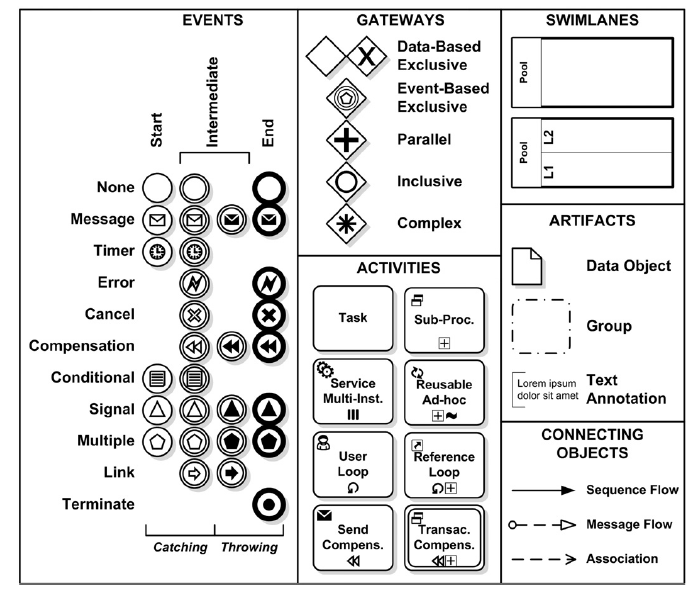
\includegraphics[scale=0.5]{images/elementos.png}
\caption{Conjunto de elementos que compõem a versão BPMN 2.0 \cite{object2016business}.}
\label{elementos}
\end{figure}

\section{Protocolos de experimentação usando BPM}

Compreender o projeto do experimento e revisar suas informações é fundamental não só para a execução do experimento, mas também para sua replicação. Diversos pesquisadores tem realizado projetos pilotos que ocasionam somente aumento de custos \cite{Kitchenham2008}. 

A utilização da notação de processo de negócio pode contribuir diretamente tanto na concepção quanto na execução do protocolo de estudo experimental. Primeiramente, devido à facilidade de compreensão do uso que compõem a respectiva notação, principalmente pelo fato de consistir em um padrão UML. Em segundo ponto, a utilização de pacotes de laboratório para o armazenamento das informações relativas aos protocolos realizados em cada experimento.

Através destes modelos de processo a seguir, é possível observar a sequência de execução das atividades, os fatores limitantes, tais como tempo, e também a estruturação de cada um dos processos e suas subdivisões.

Nas figuras \ref{selecao}, \ref{g1} e \ref{g2} são apresentados os diagramas de processo de negócio referentes ao protocolo de experimentação aplicado como parte do projeto de mestrado entitulado ``ModelUI$_{VIZ}$ - Uma proposta para representação de modelos de interface do usuário utilizando Visualização de Informação'', sob responsabilidade de Livia Cristina Gabos Martins, participante do Laboratório de Pesquisa em Engenharia de Software Aplicada -- LaPESA.

A representação do modelo de diagrama de processo de negócio também deve ser armazenado no pacote de laboratório, viabilizando o compartilhamento do protocolo juntamente com os dados referentes ao experimento, tais como hipóteses, variavéis dependentes e independentes.

%%%%%%%%%%%%%% selecao grupos
\begin{figure}[!ht]
\centering
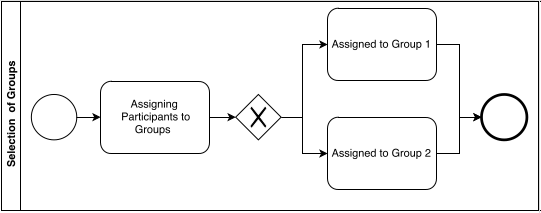
\includegraphics[scale=0.7]{images/selecao.png}
\caption{Processo de atribuição de participantes aos grupos.}
\label{selecao}
\end{figure}


\begin{landscape}

%%%%%%%%%%%%%% grupo 01
\begin{figure}[!ht]
\centering
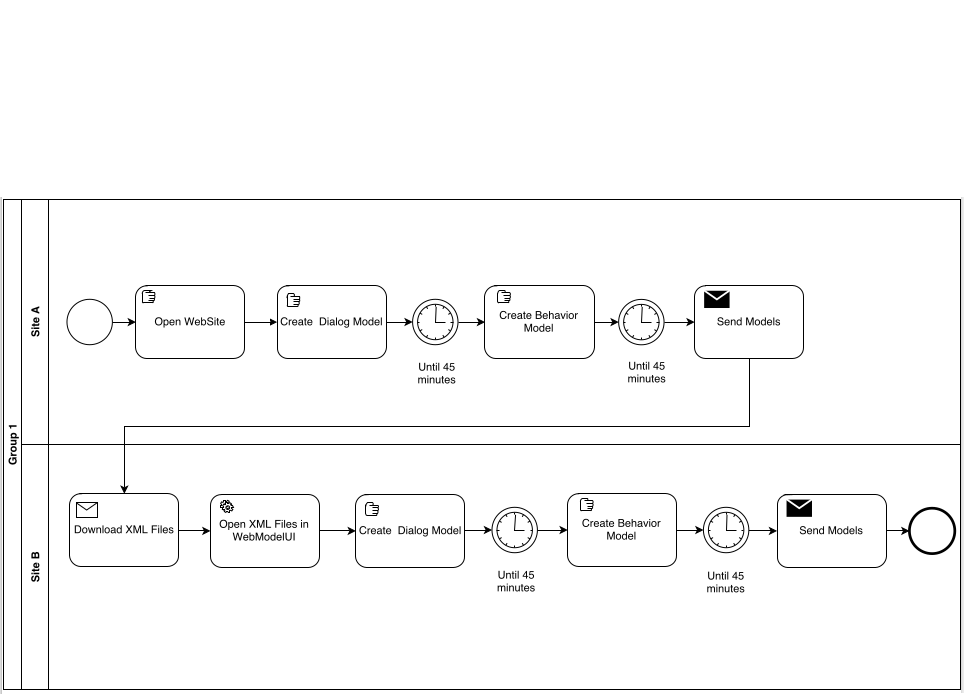
\includegraphics[scale=0.7]{images/grupo01.png}
\caption{Diagrama BPM referente às atividades dos participantes do primeiro grupo.}
\label{g1}
\end{figure}



%%%%%%%%%%%%%%% grupo 02
\begin{figure}[!ht]
\centering
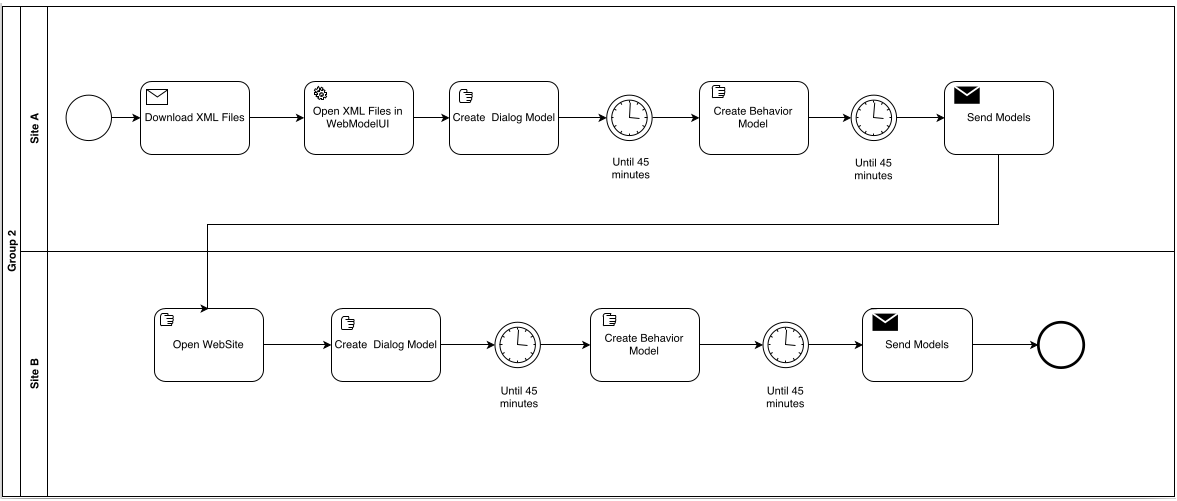
\includegraphics[scale=0.7]{images/grupo02.png}
\caption{Diagrama BPM referente às atividades dos participantes do segundo grupo.}
\label{g2}
\end{figure}


\end{landscape}





	
	\chapter{Protótipo da Interface de Modelagem}
\label{cp:prototipo}

Neste capítulo é apresentada a interface da implementação parcial (situação atual do desenvolvimento) tanto da camada de interface para modelagem gráfica quanto da camada de persistência para a notação.
Primeiramente, em relação à camada de interface, trata-se de uma plataforma \textit{web} e, para sua implementação, foram utilizados a linguagem de marcação HTML 5 (\textit{HyperText Markup Language}), o CSS 3 (\textit{Cascading Style Sheets}) e a linguagem \textit{JavaScript}. Adicionalmente, as bibliotecas \textit{JQuery} e \textit{SVGPanZoom} são utilizadas para facilitar a implementação de recursos gráficos e execução de requisições HTTP/Ajax para a comunicação com o servidor, e manipulação dos elementos gráficos por meio de de operações de escala e deslocamento, respectivamente.

A ferramenta foi projetada para ser simples e intuitiva, com foco na elaboração dos diagramas. A página inicial é apresentada na Figura~\ref{inicial}.

\begin{figure}[!htb]
\centering
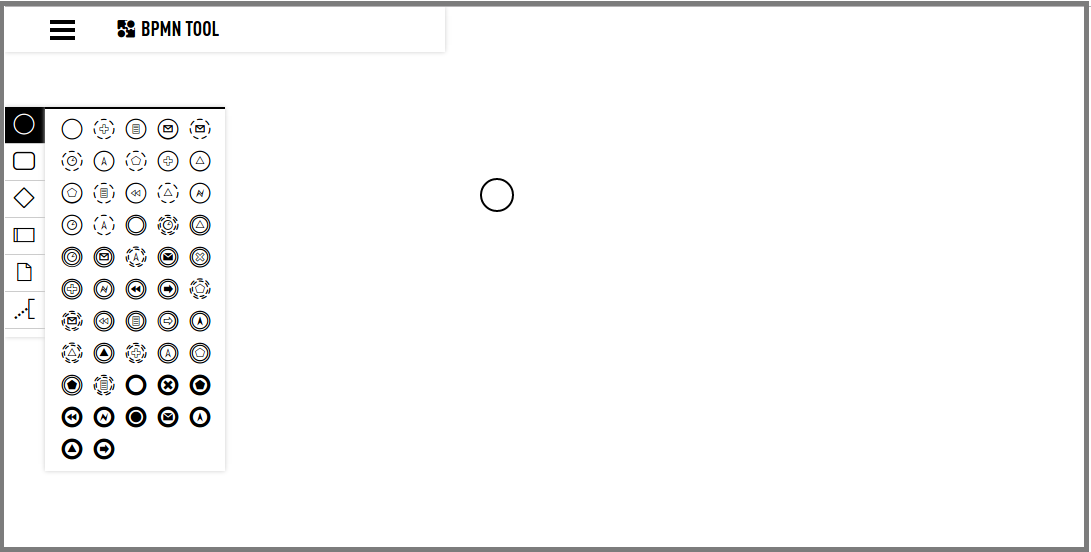
\includegraphics[width=\textwidth]{images/ferramenta.png}
\caption{Interface de modelagem da notação.}
\label{inicial}
\end{figure}

Para a criação de um novo modelo de diagrama de processo de negócio, é necessário somente realizar a inserção dos componentes do diagrama, ou caso já haja um modelo representado, o usuário deve selecionar a opção \textit{"Menu -> New"} para iniciar a representação. O menu da ferramenta é apresentado na Figura~\ref{menu}.

\begin{figure}[!htb]
\centering
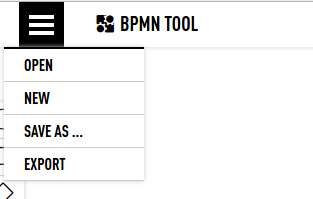
\includegraphics[scale=0.75]{images/menu.png}
\caption{Menu de opções da ferramenta.}
\label{menu}
\end{figure}

Ainda em relação à Figura~\ref{menu}, é possível observar outras opções. Na opção \textit{``Menu -> Open''}, o usuário abrir um modelo de processo de negócio elaborado previamente nesta ferramenta, armazenados em arquivos com a extensão \textit{.bpmn}. A opção ``\textit{Menu -> Save as''} permite o armazenamento do modelo no mesmo formato citado anteriormente, sendo este um diagrama concluído ou em processo de criação. Por fim, a opção \textit{``Menu -> Export''} visa armazenar o modelo em formato de imagem vetorial, no formato SVG (\textit{Scalable Vector Graphics}), de forma que, o usuário, mesmo sem acesso a esta ferramenta, possa ter acesso ao conteúdo do modelo, ao menos, para leitura de seu conteúdo.

Para a construção do modelo de processo de negócio, o usuário faz uso de elementos tais como: \textit{Events}, \textit{Gateways}, \textit{Tasks}, \textit{Pools/Lanes}, \textit{Data Objects} e \textit{TextAnnotations}. Estes elementos são encontrados na ferramenta pelo menu lateral, no qual estão presentes todos os itens dessa categorias listas anteriormente.

Na Figura~\ref{eventos}, todos os eventos e suas derivações são listados.

\begin{figure}[!htb]
\centering
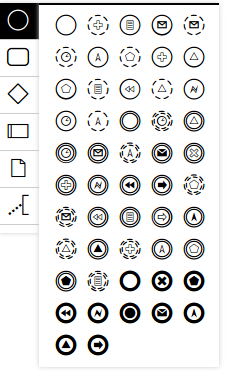
\includegraphics[scale=0.75]{images/eventos.png}
\caption{Painel de elementos da categoria de eventos.}
\label{eventos}
\end{figure}

Na Figura~\ref{gate} são apresentados os elementos que compõem a categoria de portões. E na Figura~\ref{lane} são exibidos os elementos referentes a piscinas e raias.

\begin{figure}[!htb]
\centering
\subfigure[Categoria de \textit{gateways}\label{gate}]{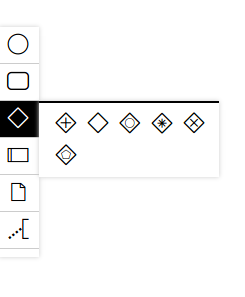
\includegraphics[scale=0.75]{images/gate.png}}\qquad\qquad
\subfigure[Categoria de piscinas e raias\label{lane}]{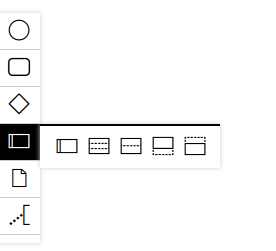
\includegraphics[scale=0.75]{images/lane.png}}
\caption{Painel de elementos}
\label{elementos}
\end{figure}
%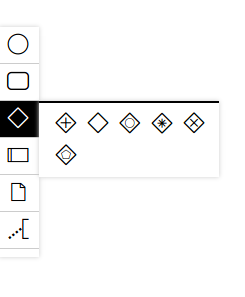
\includegraphics[scale=0.75]{images/gate.png}




Cada elemento pertencente à notação será persistido no formato XML para composição do pacote de laboratório. A figura~\ref{mensagem} representa uma tarefa da categoria de mensagens, este elemento será armazenamento no modelo apresentado na listagem~\ref{ls:message}

\begin{figure}[!htb]
\centering
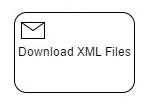
\includegraphics[scale=0.75]{images/mensagem.jpg}
\caption{Exemplo de elemento \textit{MessageTask}.}
\label{mensagem}
\end{figure}

\lstset{language=XML}
\begin{lstlisting}[caption=Descrição do elemento \textit{Mensagem}, label=ls:message]
<messagetask id="23">
	<type>task</type>
	<from>15</from>
	<to>42</to>
	<value>Download XML Files</value>
</messagetask>
\end{lstlisting}

Em relação ao servidor da plataforma \textit{web} em desenvolvimento, está sendo utilizada a linguagem de programação \textit{Java}, o servidor \textit{GlassFish Server 4.1} e o JSP - \textit{Java Server Pages}. Adicionalmente, para o suporte à serialização dos dados no formato XML (\textit{eXtensible Markup Language}) é utilizada a biblioteca \textit{XStream}. Esta parte da aplicação provê suporte tanto à leitura e escrita dos arquivos, quanto à validação dos diagramas, em termos de completude e corretitude, e também a extração do conteúdo de pacotes de laboratório e criação do respectivo modelo de processo. Aliás, a estrutura do arquivo XML deverá conter tanto elementos para representar o modelo visual BPMN (como coordenadas para posicionamento de elementos gráficos na interface), quanto elementos que representam os conceitos do Pacote de Laboratório.

Atualmente, em relação à camada de persistência, todos os elementos compõem a primeira versão da notação já foram implementados, e está em andamento a implementação dos elementos da segunda versão da notação BPM. Atualmente, foram implementadas trinta e uma classes, divididas em seis pacotes conforme a categorização dos elementos da notação. Tem sido adotada uma abordagem evolutiva, portanto os diagramas, assim como o modelo de classes, têm sido, também, alvo de contante evolução.


A seguir, na Listagem\ref{lst:classe} é apresentada a classe \textit{BusinessProcessDiagram} (apenas dados privados, que devem ser armazenados), a qual representa o componente básico de um diagrama BPMN, sendo responsável pela organização de todo o diagrama. O armazenamento desse elemento em pacote de laboratório está representado na Listagem~\ref{xml}.

\lstset{language=java}
\begin{lstlisting}[caption=Estrutura de Dados inicial da classe diagrama BPM, label=lst:classe]
public class BusinessProcessDiagram {
    private String id; 
    private String name; 
    private String version; 
    private String author; 
    private String language;  
    private String queryLanguage; 
    private Date creationDate;
    private Date modificationDate; 
    private ArrayList<Pool> pools; 
    private String documentation; 
}
\end{lstlisting}


\lstset{language=XML}
\begin{lstlisting}[caption=Estrutura do XML da classe diagrama BPM, label=xml]
<businessprocessdiagram id="1245" name="Selecao dos grupos">
  <author>Leandro Ungari</author>
  <language>pt-br</language>
  <queryLanguage>BPMN</queryLanguage>
  <creationDate>01/05/2017</creationDate>
  <modificationDate>10/05/2017</modificationDate>
  <pools>
    <pool id="1">...</pool>
    <pool id="2">...</pool>
    <pool id="3">...</pool>
         ...
    <pool id="n">...</pool>
  </pools>
  <documentation>Elemento formalizado pela documentacao BPMN 2.0 ...
	</documentation>
</businessprocessdiagram>
\end{lstlisting}





	
	\chapter{Plano inicial e atividades realizadas}
\label{ch:plano_atividades}

\section{Cronograma Inicial}
O cronograma de atividades foi organizado de acordo com a Tabela ~\ref{tab_cronograma}. As atividades foram divididas mensalmente, com início em dezembro de 2016. Nessa tabela as letras 'x' correspondem às atividades previstas e as letras 'X' às atividades já realizadas.

\begin{itemize}
\item \textit{Atividade 1}: Revisão Bibliográfica (e da tecnologia a ser utilizada);
\item \textit{Atividade 2}: Definição dos requisitos da camada de interface;
\item \textit{Atividade 3}: Desenvolvimento da camada de interface;
\item \textit{Atividade 4}: Avaliação da interface desenvolvida;
\item \textit{Atividade 5}: Relatório Parcial;
\item \textit{Atividade 6}: Relatório Final.

\end{itemize}


\begin{table}[htbp]
\centering 
\caption{Cronograma de Atividades}
\label{tab_cronograma}
\small
\begin{tabular}
{|c|c|c|c|c|c|c|c|c|c|c|c|c|} \cline{2-13}
\multicolumn{1}{c|}{}&\multicolumn{12}{c|}{\textbf{Período}}
 \\
\cline{2-13}
\multicolumn{1}{c|}{}&\multicolumn{1}{c|}{\textbf{2016}} &\multicolumn{11}{c|}{\textbf{2017}} \\
\hline Atividades & Dez & Jan & Fev & Mar & Abr & Mai & Jun & Jul & Ago & Set & Out & Nov \\
\hline         1  & X   & X   &  X  &  X  &     &     &     &     &     &     &     &     \\
\hline         2  &     &     &  X  &  X  &     &     &     &     &     &     &     &     \\
\hline         3  &     &     &     &  X  & X   &  x  &  x  & x   & x   &     &     &     \\
\hline         4  &     &     &     &     &     &     &     &     & x   & x   &  x  &  x  \\
\hline         5  &     &     &     &     &     &  X  &     &     &     &     &     &     \\
\hline         6  &     &     &     &     &     &     &     &     &     &     &   x &  x  \\
\hline
\end{tabular}
\normalsize
\end{table}

\section{Atividades Realizadas}

As atividades desenvolvidas até o presente momento foram as seguintes: foi realizada uma breve revisão bibliográfica sobre Engenharia de Software Experimental, com foco em experimentos controlados e o uso de Pacotes de Laboratório para a transferência de dados entre grupos de pesquisa, considerando o conhecimento adquirido em iniciações científicas anteriores. Em seguida, foi aprofundado o estudo em relação ao uso da notação BPM e como esta poderia ser aplicada em contexto de estudos experimentais.

Atualmente, a partir dos requisitos da camada de interface para modelagem, foi iniciada a implementação desta assim como da camada de persistência.

Em relação às próximas atividades, o próximo passo consiste em finalizar a construção da camada de persistência e da interface gráfica de modelagem. Em seguida, reaizar a integração com a ferramenta \textit{OntoExpTool} e, desta forma, avaliar o uso da notação para a construção de protocolo de experimentação. Por fim, será realizada a escrita do relatório científico final.

	
	\chapter{Considerações Finais}
\label{cp:conclusoes}

Experimentos controlados envolvem o controle de certos parâmetros para medir a influência desses em variáveis dependentes, que variam de acordo com o objeto de estudo. 

Embora sugerido na literatura, o protocolo de experimentação não é explicitado em Pacotes de Laboratório e, consequentemente, não é visível ao experimentador nem ao replicador. Desse modo, pesquisadores encontram dificuldades para estabelecer o plano de execução de um experimento, assim como, compreender o conteúdo de pacotes de laboratório para a replicação de experimentos~\cite{Wohlin2012}.

Neste trabalho foi proposta a construção de uma interface que viabilize a concepção e modelagem do protocolo do experimento, assim como o armazenamento deste conteúdo em um Pacote de Laboratório.

\section{Cronograma Inicial}
O cronograma de atividades foi organizado de acordo com a Tabela ~\ref{tab_cronograma}. As atividades foram divididas mensalmente, com início em dezembro de 2016. Nessa tabela as letras 'x' correspondem às atividades previstas, 'X' às atividades já realizadas.

\begin{itemize}
\item \textit{Atividade 1}: Revisão Bibliográfica (e da tecnologia a ser utilizada);
\item \textit{Atividade 2}: Definição dos requisitos da camada de interface;
\item \textit{Atividade 3}: Desenvolvimento da camada de interface;
\item \textit{Atividade 4}: Avaliação da interface desenvolvida;
\item \textit{Atividade 5}: Relatório Parcial;
\item \textit{Atividade 6}: Relatório Final.

\end{itemize}


\begin{table}[htbp]
\centering 
\caption{Cronograma de Atividades}
\label{tab_cronograma}
\small
\begin{tabular}
{|c|c|c|c|c|c|c|c|c|c|c|c|c|} \cline{2-13}
\multicolumn{1}{c|}{}&\multicolumn{12}{c|}{\textbf{Período}}
 \\
\cline{2-13}
\multicolumn{1}{c|}{}&\multicolumn{1}{c|}{\textbf{2016}} &\multicolumn{11}{c|}{\textbf{2017}} \\
\hline Atividades & Dez & Jan & Fev & Mar & Abr & Mai & Jun & Jul & Ago & Set & Out & Nov \\
\hline         1  & X   & X   &  X  &  X  &     &     &     &     &     &     &     &     \\
\hline         2  &     &     &  X  &  X  &     &     &     &     &     &     &     &     \\
\hline         3  &     &     &     &  X  &  X  &  X  &  X  &  X  &  X  &     &     &     \\
\hline         4  &     &     &     &     &     &     &     &     &  X  &  X  &  X  &  X  \\
\hline         5  &     &     &     &     &     &  X  &     &     &     &     &     &     \\
\hline         6  &     &     &     &     &     &     &     &     &     &     &  X  &  X  \\
\hline
\end{tabular}
\normalsize
\end{table}

\section{Atividades Realizadas}

Conforme estabelecido pelo cronograma inicial, as atividades previstas para a primeira parte do projeto, anteriores a entrega do relatório científico parcial, tinham como propósito o embasamento teórico dentro do contexto da Engenharia de Software Experimental sobre experimentos controlados, o uso de pacotes de laboratório para transferência de dados entre grupos de pesquisa. Em seguida, iniciou-se o estudo sobre modelos de processo de negócio e suas notações para representação de modelos gráficos, em específico a BPMN.

Em seguida, a partir dos requisitos da camada de interface para modelagem, foi iniciada a implementação desta ferramenta de modo a viabilizar a construção dos modelos de processo de negócio com todos os elementos previstos pela documentação da notação em sua versão atual.

Após a elaboração desta interface de modelagem, foi iniciada a construção da camada de persistência dos modelos de processo, assim como a recuperação e armazenamento destes em documentos de forma permanente. De modo análogo também foi construída uma camada de persistência e uma interface de dados para obtenção dos conteúdos relativos aos experimentos executados e armazenados segundo o modelo proposto pela ontologia \textit{ExperOntology} a partir da ferramenta \textit{OntoExpTool}. Desse modo, a partir da leitura de um pacote de laboratório é possível incorporar o modelo processo de negócio respectivo ao experimento, e assim, incorporando o protocolo de experimentação.

Em seguida, foram estabelecidas avaliações para a detecção de inconsistências tanto na ferramenta quanto na representação da notação, e desta forma, suas devidas correções. Para esta tarefa foram obtidos modelos de processos presentes na documentação oficial da notação BPMN, de forma a detectar se os modelos criados a partir ferramenta foram construídos de forma valida quanto ao conjunto de itens e seus relacionados entre elementos.

Também foram construídos alguns modelos de diagramação de forma a representar os protocolos de estudos experimentais já previamente executados para avaliar se a notação apresentada supre todas as necessidades encontradas. Em relação a instanciação de novos pacotes de laboratório, foi executado o processo de engenharia reversa a partir de um pacote de pré-existente foi elaborado o respectivo protocolo de experimental (plano de execução) e por fim, a adição do modelo de processo a nova instância do pacote de laboratório. 

Por fim, foi iniciada a construção do presente relatório científico final.

\section{Contribuições}

A principal contribuição do presente trabalho está em fornecer uma ferramenta que permita a construção e a visualização do plano de execução (protocolo) de estudos experimentais, assim como a integração desses dados a um pacote de laboratório e a vinculação do conjunto de artefatos presentes  em experimentos às suas respectivas atividades representadas por um modelo de processo de negócio.

Apesar de ter como foco a concepção do plano de execução de experimentos controlados, não foi detectada nenhuma limitação na construção de planos de execução também aos modelos de estudos experimentais (pesquisa de opinião e estudos de caso) apresentados na Seção~\ref{sect:processoexperimentacao}. Um restrição consiste na vinculação de informações do experimento, por adotar o modelo proposto na ontologia \textit{ExperOntology}. Porém, essa restrição não está relacionado a utilização de modelos de processo de negócio, mas sim pelo modelos de dados adotado.

Adicionalmente, a ferramenta também permite a manipulação de pacotes de laboratório e protocolos de experimentação sob o modelo não-relacional de dados orientado a documentos, utilizando a linguagem XML. Além da legibilidade deste formato, fornece maior portabilidade entre sistemas de software facilitando a integração de novos componentes por se tratar de um formato padrão na troca de dados, em detrimento a diversos sistemas de gerenciamento de banco de dados proprietários e com diversas restrições presentes no modelo relacional.


\section{Trabalhos Futuros}

Do ponto de vista da ferramenta desenvolvida, os seguintes aprimoramentos são desejáveis:

\begin{itemize}

\item Aprimoramento de alguns recursos gráficos da ferramenta, para uma melhor usabilidade na modelagem de processos de negócio, com a adição de recursos com redimensionamento para alguns elementos do tipo \textit{container}, assim como indicativos de seleção de itens na criação de transições.

\item Integração da camada de interface de modelagem de processo de negócio com a ferramenta de instanciação de pacotes de laboratório, viabilizando a adição de elementos a descrição do experimento por meio dos modelos gráficos \textit{OntoExpTool}.

\end{itemize}

Na perspectiva da Engenharia de Software Experimental, o próximo passo a ser feito no contexto do Grupo de Pesquisa, é apresentado a seguir como uma continuação para este Projeto de Iniciação Científica.

%%%%%%%%%%%%%%%%%%%%%%%%%%%%%%%%%%%%%%
%%%%%%%%%%%%%%%%%%%%%%%%%%%%%%%%%%%%%%
%%%%%%%%%%%%%%%%%%%%%%%%%%%%%%%%%%%%%%

\section{Proposta de Renovação}

\subsection{Contexto, Motivação e Justificativa}

Dentro do grupo de pesquisa existem experimentos conduzidos sem a definição de seus protocolos (planos de execução) utilizando a versão atual -- modelos BPMN. 
A versão atual da ferramenta, com a interface implementada neste projeto de Iniciação Científica, permite a modelagem de protocolos de experimentos usando BPMN. 

A elaboração de modelos de processo de negócio para a representação de protocolos de experimentação visa a suprir a ausência de uma visão completa sobre o plano de execução do experimento. Porém não há evidências de que o uso da notação gráfica do BPMN auxilia a construção e o entendimento, tanto quantitativa quanto qualitativa, na compreensão de experimentos e da evolução do conhecimento armazenado em pacotes de laboratório.

É preciso ter evidências dos benefícios trazidos pelo uso de BPMN no entendimento de um Pacote de Laboratório para poder indicar seu uso como uma ferramenta para a transferência de pacotes de laboratório, intra e inter-grupos. E isso justifica a proposta de continuação deste projeto de Iniciação Científica. 


%%%%=====================================================================================================
\subsection{Formulação do Problema e Objetivo do Projeto}\label{cap:objetivos}

Como exposto, o principal problema consiste na falta de padronização na organização de pacotes de laboratório, de modo a auxiliar seu entendimento. A \textit{ExperOntology} foi proposta para organizar os dados, e agora a BPMN foi implementada como uma ferramenta (camada de interface) para modelar o protocolo do experimento. Assim, o problema é avaliar (vantagens e desvantagens, se houver) do uso de BPMN como ferramenta para expor o protocolo experimental, visando a facilitar seu entendimento. 

Assim, o objetivo principal consistem em avaliar o uso da BPMN na organização e no entendimento de protocolos experimentais. Como questões de pesquisa em Iniciação Científica, tem-se: a utilização da notação auxilia a representação do protocolo do experimento? a notação facilita a identificação e a compreensão de suas atividades e artefatos utilizados?

\subsection{Metodologia e Plano de Trabalho}

Inicialmente, serão instanciados pacotes de laboratório referentes a experimentos controlados executados no âmbito do grupo de pesquisa -- registrados com a versão textual da ferramenta \textit{OntoExpTool} (sem BPMN). Esses novos pacotes de laboratório serão construídos a partir da interface de modelagem de protocolos de experimentação já implementados. Com o término desta atividade, os experimentos já executados terão seus protocolos modelados em BPMN.  

Após a criação dos protocolos em BPMN, será feita uma revisão deles pelos autores dos experimentos originais para detectar possíveis inconsistências e incoerências. Na impossibilidade de um autor participar, o orientador revisará os protocolos. 

Uma vez aprovados pelos autores originais, os protocolos expressos em BPMN serão avaliados por terceiros. Será feito um experimento, no qual um protocolo (modelo BPMN de um experimento) será fornecido para um avaliador, que deverá descrever o experimento para verificar se, de fato, entendeu seu conteúdo. Autores de um experimentos atuarão como avaliadores de outro experimento, além de alunos do Programa de Mestrado em Ciência da Computação da UNESP (os alunos de mestrado farão tal avaliação do protocolo como parte de uma disciplina).

A última atividade consiste em analisar os resultados obtidos para que seja escrito um artigo científico.

Paralelamente às tarefas citadas anteriormente, serão redigidos o relatório parcial e final, conforme exigido. 
\begin{table}[htbp]
\centering \caption{Cronograma de Atividades}\label{tab_cronograma2}
%\small
\begin{tabular}
{|c|c|c|c|c|c|c|c|c|c|c|c|c|} \cline{2-10}
\multicolumn{1}{c|}{}&\multicolumn{9}{c|}{\textbf{Período em meses}}
 \\
\cline{2-10}
\hline Atividades & 1   & 2   & 3   & 4   & 5   & 6   & 7   & 8   & 9   \\
\hline         1  & X   & X   &     &     &     &     &     &     &     \\
\hline         2  &     &     &  X  &     &     &     &     &     &     \\
\hline         3  &     &     &     &     &  X  &  X  &     &     &     \\
\hline         4  &     &     &     &     &     &     &  X  &  X  &     \\
\hline         5  &     &     &     &  X  &     &     &     &     &     \\
\hline         6  &     &     &     &     &     &     &     &  X  & X   \\
\hline
\end{tabular}
\normalsize
\end{table}
%%%%%%%%%%%%%%
Na Tabela~\ref{tab_cronograma2} é apresentado o cronograma proposto com a duração expressa em meses, sendo que as atividades descritas foram agrupadas como segue: 

\begin{enumerate}
\item Empacotamento dos experimentos;
\item Revisão dos pacotes de laboratório;
\item Avaliação dos pacotes de laboratório;
\item Análise de resultados e elaboração do artigo científico;
\item Relatório Parcial;
\item Relatório Final.
\end{enumerate}





	% ----------------------------------------------------------
	% ELEMENTOS PÓS-TEXTUAIS
	% ----------------------------------------------------------
	\postextual
	% ----------------------------------------------------------

	% ----------------------------------------------------------
	% Referências bibliográficas
	% ----------------------------------------------------------
\renewcommand{\bibname}{Referências Bibliográficas}
%\addcontentsline{toc}{chapter}{Referências Bibliográficas}
\bibliography{referencias/referencias}

	
\end{document}
